%_______________________________________________________________________________
%class
%_______________________________________________________________________________
%\documentclass[a4paper,11pt,onecolumn,final,german,openbib]{scrbook}
\documentclass[a4paper,11pt,oneside,final,german,openbib,pdftex]{scrbook}
%_______________________________________________________________________________
% page borders
%_______________________________________________________________________________
\addtolength{\headheight}{2cm}
%\addtolength{\topmargin}{2cm}
\setlength{\oddsidemargin}{1.0cm}
\setlength{\evensidemargin}{0.5cm}
\setlength{\textwidth}{14.3cm}
\setlength{\parindent}{0mm}

% Default folder for graphics
 
%_______________________________________________________________________________
% packages
%_______________________________________________________________________________
\usepackage{german}
\usepackage{amsmath, amssymb}
\usepackage[utf8]{inputenc}
\usepackage{graphicx}
\usepackage{enumerate}
\usepackage{multirow}
\usepackage{subfigure}
\usepackage{dsfont}
\usepackage{slashed} 
\usepackage{textcomp}
\usepackage{svg}
\usepackage{pdfpages}
\usepackage{placeins}
\usepackage{float}
\usepackage[labelfont=bf, format=plain]{caption}
\usepackage{cite}



%_______________________________________________________________________________
% bold fonts for headings
%_______________________________________________________________________________
\font\afont=cmssbx10 scaled \magstep5     % for the title
\font\bfont=cmssbx10 scaled \magstep4     % for chapter headings
\font\cfont=cmssbx10 scaled \magstep3
\font\dfont=cmssbx10 scaled \magstep2     % for section headings and author name
\font\efont=cmssbx10 scaled \magstephalf

%_______________________________________________________________________________
% index depth
%_______________________________________________________________________________
\setcounter{secnumdepth}{3}
\setcounter{tocdepth}{3}

%_______________________________________________________________________________
% new commands
%_______________________________________________________________________________
\newcommand{\demi}{\frac{1}{2}}

%_______________________________________________________________________________
% renewed commands
%_______________________________________________________________________________
% \renewcommand{\topfraction}{1.}       % this is important for figure placement
% \renewcommand{\bottomfraction}{1.}
\makeatletter
\renewcommand\paragraph{\@startsection{paragraph}{4}{\z@}%
  {-3.25ex\@plus -1ex \@minus -.2ex}%
  {1.5ex \@plus .2ex}%
  {\normalfont\normalsize\bfseries}
}
\makeatother


%_______________________________________________________________________________
% special words, hyphenation
%_______________________________________________________________________________
\hyphenation{Ba-che-lor-ar-beit}


\pagestyle{empty}
\pagestyle{headings}
%for changing the style on a specific page use \thispagestyle{e.g., empty}

%_______________________________________________________________________________
%_______________________________________________________________________________
\begin{document}
\pagenumbering{roman}

%_______________________________________________________________________________
% \begin{titlepage}
%   \vspace*{6mm}
%   \begin{center}
%      {\afont Rastertunnelmikroskopie an adsorbierenden Schichten}
%      \\[3.5cm]
%      {\large von}
%      \\[3.5cm]
%      {\dfont Verena Grimm}
%      \\[2cm]
%      {\large Bachelorarbeit in Physik \/\\
%         vorgelegt dem Fachbereich Physik, Mathematik und Informatik (FB 08) \/\\
%         der Johannes Gutenberg-Universit\"at Mainz \/\\
%         am 03. Juni 2014}
%    \end{center}
%    \vfill
%    1. Gutachter: Prof. Dr. Hans-Joachim Elmers\\	
%    2. Gutachter: Prof. Dr. ?????????????????? \\
%    \vfill
% \end{titlepage}

% \thispagestyle{empty}
% Ich versichere, dass ich die Arbeit selbstst\"andig verfasst und keine 
% anderen als die angegebenen Quellen und Hilfsmittel benutzt sowie 
% Zitate kenntlich gemacht habe.
% \\
% \\[3.5cm] 
% Mainz, den [Datum] [Unterschrift]
% \vfill
% \noindent 
% Verena Grimm\\
% KOMET\\
% Institut f\"ur Physik\\
% Staudingerweg 7\\
% Johannes Gutenberg-Universit\"at
% D-55128 Mainz\\
% {\tt vegrimm@students.uni-mainz.de}

%_______________________________________________________________________________
\renewcommand\contentsname{Inhaltsverzeichnis}
\renewcommand\figurename{Abbildung}
\renewcommand\tablename{Tabelle}
\tableofcontents
\clearpage 

\mainmatter  
\sloppy

%_______________________________________________________________________________
% \chapter{Einleitung}





%_______________________________________________________________________________
\chapter{Hauptteil}


%_______________________________________________________________________________
\section{Grundlagen}

% \subsection{Oberflächenstrukturen}
% Im folgenden werden die Oberflächenstrukturen von Festkörpern mit periodischem Aufbau näher
 beleuchtet. \\
 Betrachtet man die Oberfläche eines solchen Festkörpers, so ist leicht einsehbar, dass die
 Kräfte zwischen Atomen der äußersten Schicht durch fehlende Nachbarn auf einer Seite beträchtlich
 anders sind. Die Gleichgewichtsbedingungen der Oberflächenatome sind im Vergleich zum
 Körperinneren geändert, sodass man in der Regel andere Positionen der Atome und eine andere Oberflächenstruktur
 als im Inneren erwartet. Die Oberfläche ist in diesem Sinn nicht einfach wie ein (gedanklicher)
 Schnitt durch den Kristall.\\
 Verbreitete Veränderungen sind zum Beispiel die Relaxation und die Rekonstruktion. Bei der
 Relaxation bleibt die Periodizität des zweidimensionalen Gitters die Gleiche wie die der
 körperinneren Schichten, jedoch ist der Abstand dieser Schicht zu der
 darunterliegenden kleiner, seltener auch größer (siehe Abb. \ref{blabla}). Die Rekonstruktion
 beschreibt Verschiebungen parallel zur Oberfläche. Dabei kann sich die Größe der
 zweidimensionalen Einheitszelle verändern, aber auch deren Lage hinsichtlich der darunterliegenden
 Schichten (z.B. Drehungen) oder ihre Gestalt.  Beispielsweise rekonstruiert Gold die
 (100)-Oberfläche von einer fcc-Struktur zu einer hcp-Struktur. [Quelle?] Weiterhin können Atome
 oder ganze Reihen von Atomen auf der Oberfläche fehlen im Vergleich zum Inneren. 
\subsection{Rastertunnelmikroskopie}
Das Rastertunnelmikroskop (engl. Scanning Tunneling Microscope, kurz: STM) ist eine Variante der
Rastersondenmikroskopie, bei der eine dreidimensionale Aufnahme von Oberflächen elektrisch
leitender Festkörper erstellt werden kann. Dabei ist eine Afulösung auf atomaren Niveau möglich. Die
Funktionsweise beruht auf dem quantenmechanischen Tunneleffekt (siehe Abb. \ref{tunnel}): Wird eine
sehr feine, leitende Spitze bis auf wenige {\AA} an die Oberfläche heran gebracht und eine Spannung
von etwa 1V angelegt, fließt zwischen Spitze und Oberfläche ein Strom von wenigen nA. Durch
die kurze Distanz ist die Tunnelbarriere, die das Vakuum darstellt, endlich, und je nach Polung der Spannung können
die Elektronen von der Spitze zur Oberfläche tunneln bzw.
umgekehrt. Der Strom ist dabei abhängig vom Abstand, von der elektronischen Zustandsdichte der
Spitze und der Probe an dieser Stelle sowie von der angelegten Spannung. Wird die Spitze
über die Oberfläche bewegt und Strom bzw.
Abstand gemessen, kann auf diese Weise ein topographisches Bild der Oberfläche mit atomarer
Auflösung erreicht werden. 

\begin{figure}[H]
\centering
\sffamily 
\includesvg[svgpath=theorie/]{tunnel}
\caption{\textit{Veranschaulichung des Tunneleffekts. Ein Elektron mit Energie $E_{e^-}$ kann nach
klassischen Gesetzen die Potentialbarriere $V$ mit $V>E_{e^-}$ nicht überwinden, tatsächlich besteht
jedoch nach quantenmechanischer Rechnung eine endliche Wahrscheinlichkeit dafür, das Teilchen
außerhalb der Barriere zu finden. Das Elektron durchtunnelt diese, wobei die
Aufenthaltswahrscheinlichkeit $|\Psi|^2$ innerhalb der Barriere exponentiell abklingt. }}
\label{tunnel}
\end{figure}


Eine der größten Hindernisse bei der quantitativen Beschreibung der Rastertunnelmikroskopie ist die
im Allgmeinen unbekannte Struktur der Spitze, sodass eine Beschreibung immer Annahmen und Näherungen
beinhaltet. Einer dieser Näherungen ist die von Tersoff und Hamann \cite{Ter83}, \cite{Ter85}, die
zu einer direkten Interpretation der STM Bilder als konstante lokale Oberflächenzustandsdichte führt.\\
Der Strom ist nach Störungstheorie erster Ordnung nach Bardeen \cite{Bar} gegeben durch

\[I=\frac{2\pi e}{\hbar}\sum_{S,P}
f(E_{S})[1-f(E_{P}+eU)]\cdot|M_{SP}|^2\delta(E_{S}-E_{P})\]

mit der Fermifunktion $f(E)$, der angelegten Spannung $U$, der Energie
$E_{S}$ des Zustandes $\psi_{S}$ ohne Tunneln sowie dem Tunnelmatrixelement $|M_{SP}|$
zwischen den Zuständen $\psi_{\mu}$ der Spitze und $\psi_{\nu}$ der Oberfläche

\[M_{SP}=-\frac{\hbar^2}{2m}\int d\vec{S}\cdot(\psi_{S}^*\nabla\psi_{P} -
\psi_{P}\nabla\psi_{S}^*) \]

wobei die Fläche $d\vec{S}$ dabei vollständig innerhalb der Vakuumbarriere liegen muss, die
Spitze und Probe trennt. Mit der Näherung kleiner Temperaturen und kleiner Spannungen $U$ ergibt
sich

\[I=\frac{2\pi e^2}{\hbar}U\sum_{S,P}|M_{SP}|^2\delta(E_{P}-E_{F}) \delta(E_{S}-E_{F})\]

mit der Fermienergie $E_F$. Da die Wellenfunktion $\psi_{\mu}$ der Spitze unbekannt ist, wird sie
nun folgendermaßen modelliert: Der Teil der Spitze, der der Oberfläche am nächsten ist, wird als
sphärischer Potentialtopf angesetzt (siehe Abb. \ref{spitze}). Dabei ist $R$ der Radius der Kugel
und $d$ ist der kürzeste Abstand zur Oberfläche. Das Matrixelement $|M_{SP}|$ wird
also lediglich für ein s-Orbital der Spitze ausgewertet, die d- und p-Wellenfunktionen werden
vernachlässigt. Weiterhin wird vereinfachend angenommen, dass die Austrittsarbeit von Spitze und
Probe gleich ist.

\begin{figure}[H]
\centering
\sffamily 
\includesvg{spitze}
\caption{\textit{Schema des Tunnelkontakts nach Tersoff und Hamann. Die Spitze wird als sphärisches
Potential mit Radius $R$ und Abstand $d$ zur Probenoberfläche modelliert.}}
\label{spitze}
\end{figure}
 
 Die explizite Rechnung soll hier nicht ausgeführt werden (für Details, siehe \cite{Ter83}).
 Letztendlich erhält man für den Tunnelstrom $I$
 
 \[I=32\pi^3\hbar^{-1}e^2U\phi^2\rho_{S}(E_F)R^2\kappa^{-4}e^{2\kappa
 R}\cdot\rho_P(\vec{r}_0, E)\]
 
 mit der Zustandsdichte $\rho_{S}$ pro Volumen der Spitze, der Austrittsarbeit $\phi$, der inversen
 Abklinglänge $\kappa=\hbar^{-1}(2m\phi)^{1/2}$ sowie der Zustandsdichte der Probe
 $\rho_P(\vec{r}_0, E)$
 
 \[\rho_P(\vec{r}_0, E)=\sum_{P}|\psi_{P}(\vec{r}_0)|^2\delta(E_{P}-E_F).\]
 
 Wie erwartet gilt also
 
 \[I\propto U \rho_{s}(E_F) \rho_P(\vec{r}_0, E).\]
 
 Der Zusammenhang zum Abstand zwischen Probe und Spitze ergibt sich aus der
 Wellenfunktion der Probe, die im Vakuum exponentiell abfällt:
 
 \[|\psi_P(\vec{r}_0)|^2\propto e^{-2\kappa(d+R)}~~~\Rightarrow~~~I\propto e^{-2\kappa d}\]
 
% ok was weiß ich?
% - das mit der auflösung passt noch nicht so ganz, aber das kommt daher, weil die nur s orbitale
% betrachtet haben, was besser wird wenn man d und p orbitale mit dazunimmt, und außerdem das
% effektive potential, was binnig vorgeschlagen hat
\subsection{LEED-Untersuchung}
\FloatBarrier

Eine einfache und verbreitete Methode, um etwas über Oberflächenstrukturen von
 Kristallen herauszufinden, ist eine Untersuchung der Oberfläche mit LEED (Low Energy Electron
 Diffraction).
 Dabei wird ein Elektronenstrahl mit einer Energie von \SIrange{20}{400}{eV} senkrecht auf die
 Oberfläche gerichtet. Aus dem resultierenden
 Beugungsmus\-ter der elastisch rückgestreuten Elektronen, die als helle Punkte (Spots) auf einem 
 fluoreszierenden Schirm zu sehen sind, können Rückschlüsse auf die Periodizität des Gitters gezogen werden.
 \\
  Abbildung \ref{leedaufbau} zeigt den prinzipiellen Versuchsaufbau einer LEED-Vorrichtung. Die
 Elektronenkanone besteht aus einem Thorium-beschichteten Iridium-Filament, das durch Glühemission
 Elektronen emittiert. Mit Hilfe eines Wehneltzylinders kann die Fokussierung
 des Elektronenstrahls reguliert werden. Vor dem halbkugelförmigen Schirm befinden
 sich vier ebenso geformte Gitter, durch die inelastisch gestreute Elektronen mit wesentlich
 niedrigeren Energien davon abgehalten werden, auf dem Schirm störendes Hintergrundleuchten zu
 verursachen; zudem dienen auch sie der Fokussierung. Der Schirm selbst ist positiv geladen, um
 die elastisch gestreuten Elektronen auf dem letzten Weg zum Schirm zu beschleunigen.
 \\
  Da die mittlere freie Weglänge solch niederenergetischer Elektronen in
 Festkörpern sehr gering ist, dringen sie nur in die obersten Schichten des
 Kristalls ein. Damit ist diese Untersuchungsmethode sehr oberflächensensitiv.

 \begin{figure}[htbp]
	\centering
	\sffamily 
	\includesvg[svgpath=theorie/]{leed}
	\caption{\textit{Schema des LEED-Aufbaus. Die am Filament emittierten Elektronen werden an der
	Probenoberfläche gebeugt. Inelastisch gestreute Elektronen mit nied\-rig\-erer Energie werden durch
	die Gitter abgebremst, die elastisch gestreuten Elektronen dagegen werden zum Leuchtschirm
	hin beschleunigt. Dort kann dann das Beugungsbild beobachtet werden. In der Skizze sind nur zwei
	Gitter angedeutet, tatsächlich sind im verwendeten Aufbau vier Gitter verbaut.}}
	\label{leedaufbau}
\end{figure}

 Die Wellenlänge $\lambda$ der Elektronen mit Energie $E$ und Masse $m$ liegt im Bereich des
 Gitterabstandes und berechnet sich über die deBroglie Beziehung:
 
 \[\lambda=\frac{h}{\sqrt{2mE}}.\]%\approx \sqrt{\frac{1{,}5}{E_{eV}}}\]
 
Um das Beugungsmuster zu verstehen, betrachtet man vereinfacht eine elastische
Streuung nur an der obersten Atomschicht. Im Falle der elastischen Streuung ist
der Betrag des ausfallenden Wellenvektors $\vec{k'}$ gleich dem des
einfallenden Vektors $\vec{k}$, also $k=k'$. Für konstruktive Interferenz
muss die Laue-Bedingung erfüllt sein:

\[\vec{k}-\vec{k'}=\Delta \vec{k}=\vec{G}\]

mit dem reziproken Gittervektor $\vec{G}$, genauso wie die Laue-Gleichungen

\begin{equation}
\vec{a}_i\cdot \Delta \vec{k}=2\pi h_i,~~~~~~~i=1, 2, 3,
\label{gleichung}
\end{equation}

wobei $\vec{a}_i$ die primitiven Gittervektoren des Realraums und $h_i$ die Millerschen Indizes
sind. In diesem Fall der Oberflächenstreuung erhalten wir konstruktive Interferenz,
wenn die Vektorkomponten parallel zur Oberfläche, $\Delta\vec{k}_{||}=\vec{k}_{||}-\vec{k'}_{||}$,
einem reziproken Gittervektor der zweidimensionalen Oberfläche entspricht. Senkrecht zur Probenoberfläche
gibt es keine solche Beugungsbedingung. Möchte man nun die Ewald-Konstruktion auf dieses
zweidimensionale Problem anwenden, muss die dritte Laue-Gleichung (\ref{gleichung}) fallen gelassen
werden.
Statt diskreter Punkte in der dritten Dimension werden nun jedem Gitterpunkt ($h_1, h_2$) durchgehende
Linien senkrecht zur Oberfläche zugewiesen. Veranschaulicht ist diese Konstruktion in Abb.
\ref{ewald}. Der einkommende Strahl mit Wellenvektor $\vec{k}$ wird mit seiner Spitze auf einem
reziproken Gitterpunkt positioniert, sein Anfang dient als Mittelpunkt der Ewaldkugel. Die
Bedingung $\Delta \vec{k}_{||}=\vec{G}_{||}$ ist nun für jeden Punkt erfüllt, an dem die Kugel eine
der Linien schneidet. 

\begin{figure}[H]
\centering
\sffamily 
\includesvg[svgpath=theorie/]{ewald}
\caption{\textit{Die Konstruktion der Ewaldkugel einer elastischen Streuung an einer
zweidimensionalen Oberfläche. Die reziproken Gitterpunkte} (hk) \textit{sind auf einer Achse $k_x$
eingezeichnet. Die Bedingung für konstruktive Interferenz, $\Delta \vec{k}_{||}=\vec{G}_{||}$,  ist erfüllt, wo die Kugel eine der senkrechten Linien
schneidet, z.B. bei $(30)$. }}
\label{ewald}
\end{figure}

Bei einer realen Streuung muss natürlich auch die Streuung der Elektronen an tief\-eren
Schichten berücksichtigt werden, sodass die dritte Laue-Bedingung nicht komplett fallen gelassen werden
kann. Je tiefer die Elektronen in den Kristall eindringen, desto mehr Beugungseffekte senkrecht zur
Oberfläche tragen zum Beugungsbild bei, desto wichtiger wird also die Laue-Gleichung für diese
Dimension. Nicht zu vernachlässigen sind außerdem mehrfach gestreute Elektronen, Störungen in der
Oberflächenstruktur wie Defekte oder Verschmutzungen, sowie inelastisch gestreute Elektronen, die in
dieser simplen Konstruktion nicht mit einbezogen werden. Im Aufbau können diese jedoch durch die
Gitter größtenteils herausgefiltert werden. Näheres zu einer dynamischen Theorie der
Elektronenbeugung in LEED findet sich in \cite{Lueth}.

\FloatBarrier













% \section{Versuchsaufbau} 
% \subsection{Aufbau der UHV-Apparatur}

Der Sprühbeschichter wurde auf der bisher vorhandenen Ultrahochvakuums-Apparatur (siehe Abb \ref{uhvaufbau})
aufgebaut.
Diese besteht aus mehrerern Kammern, die untereinander verbunden sind. Die gesamte Apparatur ist auf vier
Druckluftfüßen gelagert, um über den Boden übetragende störende Schwingungen zu minimieren. Um ein
Ultrahochvakuum im Bereich von $10^(-10)$ zu erzeugen, kann die Apparatur zunächst mit einem mobilen Pumpstand 
(blablabla pumpe) auf Hochvakuum im Bereich von $10^{-xyz}$ gepumpt werden; ab einem Druck von $10^-6$ lässt
sich die Ionengetterpumpe hinzuschalten.\\
Die Apparatur besteht im wesentlichen aus drei wichtigen Kammern (siehe Abb. \ref{img:uhvkammern}): der 
Molekülkammer (1), der STM-Kammer (2) und der Hauptkammer (3). In der Molekülkammer kann die eingebrachte
Probe mit Hilfe des Molekülverdampfers (der in dieser Arbeit nicht zum Einsatz kam) bedampft werden. Im Rahmen
dieser Arbeit wurde der Sprühbeschichter auf die Molekülkammer aufgesetzt. In der STM-Kammer kann die Probe
mittels Rastertunnelmikroskopie- und spektroskopie untersucht sowie geflasht werden. Die Haupkammer dient zur
Untersuchung der Probe durch LEED, weiterhin kann hier durch einen unten in der Kammer eingebauten
Metallverdampfer selbige mit verschiedenen Metallen bedampft werden (Gold, Eisen, Kobalt). Auch hier ist ein
Flashen der Probe möglich über ein Heizfilament am sogenannten Manipulator, in dem die Probe gehalten wird.
Der Manipulator ermöglicht ein Drehen sowie iein Verschieben der Probe in x-z-Richtung.\\



\subsection{Aufbau des Sprühbeschichters}

Der Sprühbeschichter funktioniert im wesentlichen über ein Druckgefälle innerhalb seines Aufbaus, durch das
die in einer Lösung gelösten Moleküle auf das Substrat "`gesaugt"' werden und sie dort im besten
Falle haften bleiben. \\
Ein Schema des Aufbaus ist in Abb. \ref{aufbau} zu sehen. Ganz oben befindet sich ein elektrisch
gesteuertes Ventil, in dessen Behältnis (?) sich die Suspension befindet. Dieses Ventil wird über eine
Steuerungseinheit mit verschiedenen einstellbaren Öffnungsmodi bedient (siehe Abschnitt \ref{kaptest}). Ist es
geöffnet, wird die Suspension durch die 1mm große Öffnung in den darunterliegenden, vakuumierten Würfel
gesogen. Das Vakuum in diesem Würfel wird durch einen an einer Seite angeschlossenen Pumpstand hergestellt
und soll idealerweise im Bereich von $10^{-5}$mbar liegen. Im Würfel befindet sich ein metallischer
Konus, dessen Spitze eine Öffnung von wiederum 0,1mm aufweist. Er ist die Verbindung zwischen Würfel und dem
unteren Teil des Aufbaus, der auf der Molekülkammer aufgesetzt ist und einen Druck im Bereich von
$10^{-8}$mbar aufweisen sollte.  
Seine Aufgabe ist, dafür zu sorgen, dass einerseits nur ein dünner Strahl der eingelassenen Suspension in
den unteren Teil des Aufbaus gelangt, damit sich die Moleküle gleichmäßig auf dem Substrat verteilen und
nicht in Tröpfchen. Gleichzeitig soll er durch seine kleine Öffnung einen schnellen Druckausgleich zwischen
dem unteren Teil und dem Würfel verhindern. \\
Weiterhin sind zwei weitere Ventile in dem Aufbau enthalten. Mit Ventil 1 kann der Würfel von der
Molekülkammer abgetrennt werden. Dies kann man nutzen, um Würfel oder das elektrische Ventil zu säubern, ohne
dabei der kompletten vorderen Teil der Kammer belüften zu müssen. Wird der Würfel dann bei geschlossenem
Ventil 1 erneut über den Pumpstand vakuumiert, kann Ventil 2 geöffnet werden, damit auch das Verbindungsstück
unterhalb des Würfels über Schlauch und T-Stück mitgepumpt werden kann und nicht nur über die kleine Öffnung
des Konus.\\
Das zweite Verbindungsstück ist eine Überbrückung zwischen Ventil 1 und Adapterflansch, mit dem
der 40mm-Anschluss von Ventil 1 %bzw. des zweiten Verbindungsstückes 
auf die 63mm-Öffnung der Molekülkammer gesetzt werden kann. Eine direkt Verbindung zwischen diesem
Ventil und dem Adapter war nicht möglich, da beide ein geschlossenes Gewinde (?) besitzen.\\
Unten in der Molekülkammer befindet sich das Substrat. Die durch den Konus in den unteren Teil des Aufbaus
gelangten Moleküle sollten sich in der restlichen Kammer verteilen und auf dem Substrat zu liegen kommen.

% An einer Seite des Würfels ist ein Pumpstand angeschlossen, der ein Vakuum im
% Bereich von $10^{-5}$mbar herstellen soll. Der Teil unterhalb des Würfels ist mit der Molekülkammer
% verbunden und wird über die Getterpumpe vakuumiert. Lediglich zu Beginn, wenn der Pumpstand
% hochgefahren wird, kann das zweite Ventil geschlossen und das erste geöffnet werden, sodass das
% erste Verbindungsstück direkt unterhalb des Würfels über Schlauch und T-Stück ebenfalls gepumpt werden
% kann.\\
% Das erste Ventil dient auch dazu, den Würfel von der Kammer trennen zu können, falls dieser
% oder das Ventil für die Suspension gereinigt werden müssen. Auf diese Weise muss nicht der ganze
% vordere Teil der Vakuumkammer, sondern nur der Würfel belüftet werden.\\




 
\section{Aufbringen dünner Au-Schichten auf einem Re-Kristall}
\FloatBarrier


\begin{figure}[htbp]
	\begin{minipage}[b]{0.5\textwidth} 
		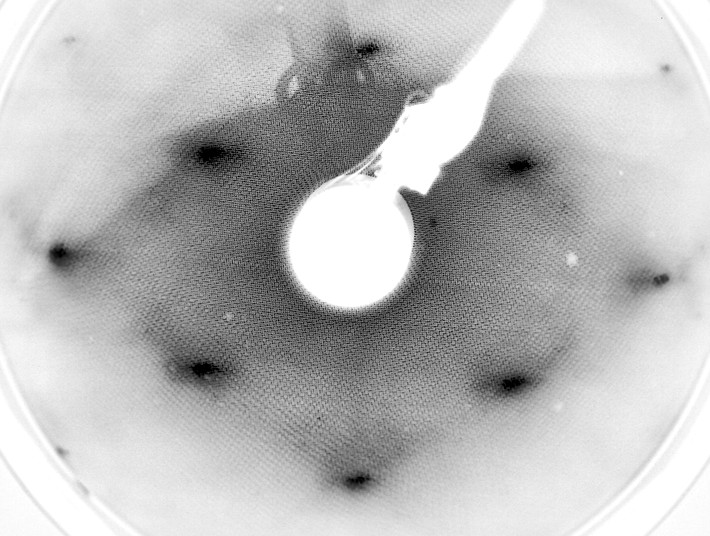
\includegraphics[width=\textwidth]{LEED-Bilder/bearbeitet/unbedampft_E207}
		\label{Bild} 
	\end{minipage}
	\hfill
	\begin{minipage}[b]{0.5\textwidth}
		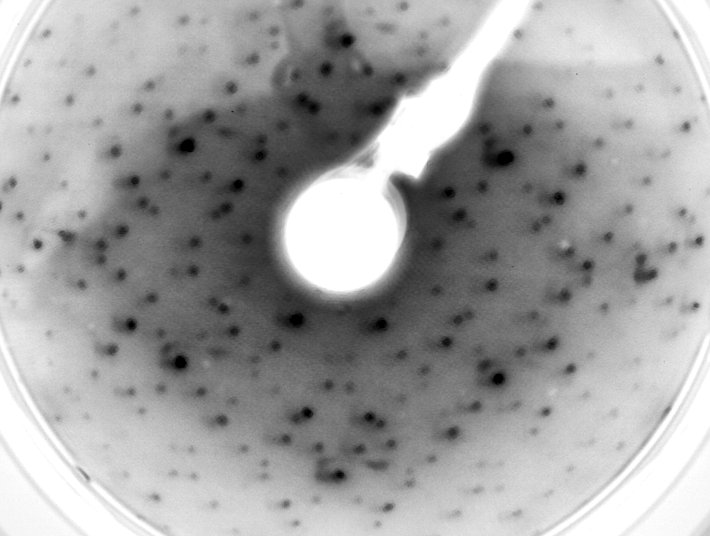
\includegraphics[width=\textwidth]{LEED-Bilder/bearbeitet/unbedampft_E207_MitteKristall.jpg}
		\label{Bild} 
	\end{minipage}
	\caption{\textit{Links der Re-Kristall mit scharfen Spots und eindeutiger Struktur. Rechts die
	Re-Oberfläche mit Verschmutzung, zu erkennen an der Überstruktur und den schwächeren Hauptspots.}}
\end{figure}

\begin{figure}[htbp]
		\captionsetup{name=Abb.}
	\begin{minipage}[b]{0.5\textwidth} 
		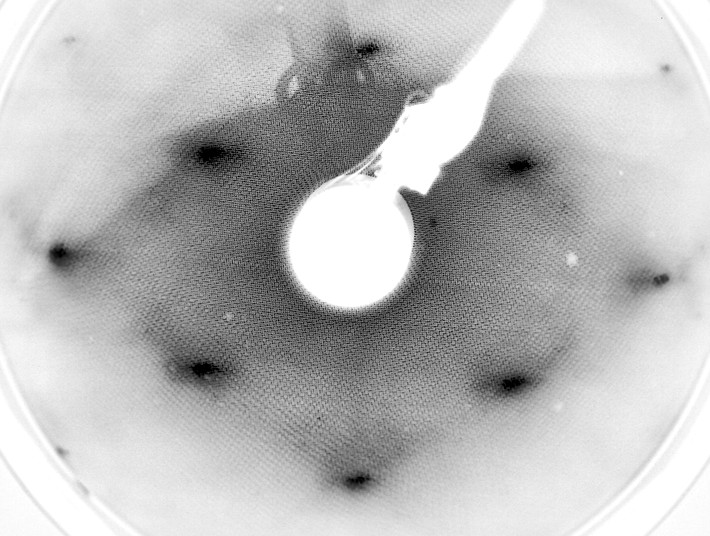
\includegraphics[width=\textwidth]{LEED-Bilder/bearbeitet/unbedampft_E207}
		\caption{\textit{Re-Oberfläche}}
		\label{Bild} 
	\end{minipage}
	\hfill
	\begin{minipage}[b]{0.5\textwidth}
		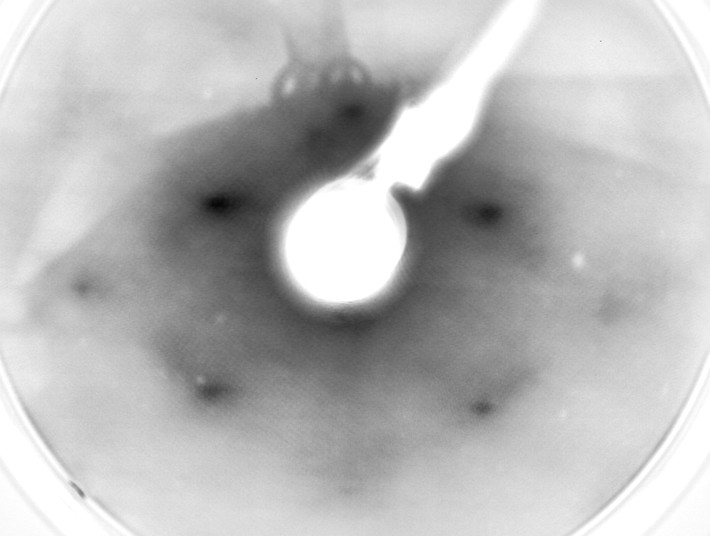
\includegraphics[width=\textwidth]{LEED-Bilder/bearbeitet/0_5ML_E208}
		\caption{\textit{1/2 Monolage Au}}
		\label{Bild} 
	\end{minipage}
	
	\begin{minipage}[b]{0.5\textwidth} 
		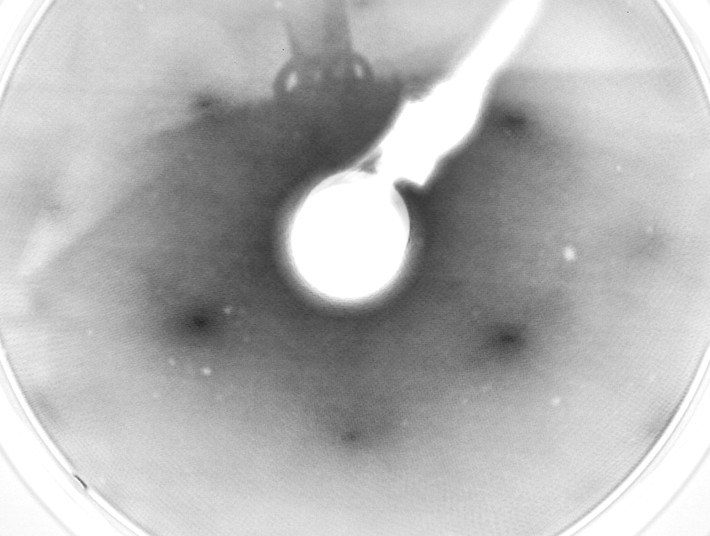
\includegraphics[width=\textwidth]{LEED-Bilder/bearbeitet/1ML_E207}
		\caption{\textit{1 Monolage Au}}
		\label{Bild} 
	\end{minipage}
	\hfill
	\begin{minipage}[b]{0.5\textwidth}
		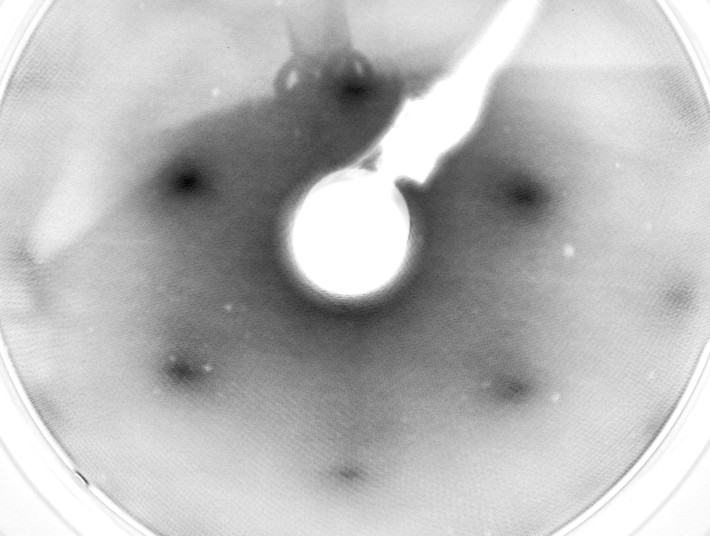
\includegraphics[width=\textwidth]{LEED-Bilder/bearbeitet/6ML_E207}
		\caption{\textit{6 Monolagen Au}}
		\label{Bild} 
	\end{minipage}
	
	\begin{minipage}[b]{0.5\textwidth} 
		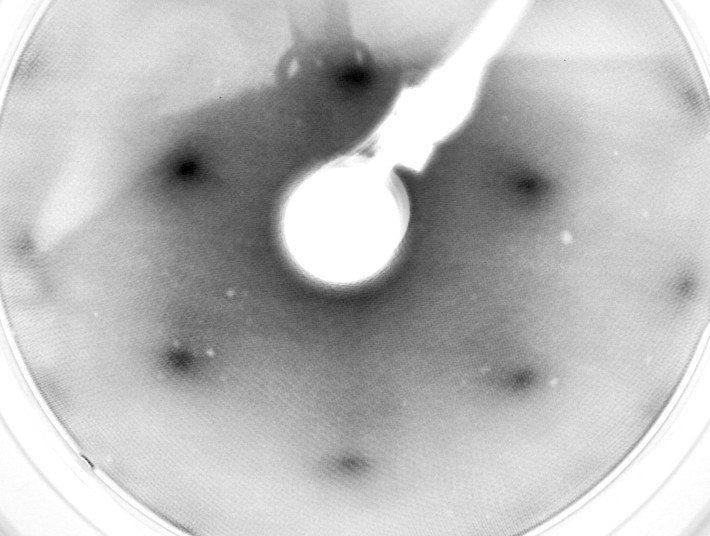
\includegraphics[width=\textwidth]{LEED-Bilder/bearbeitet/10ML_E207}
		\caption{\textit{10 Monolagen Au}}
		\label{Bild} 
	\end{minipage}
	\hfill
	\begin{minipage}[b]{0.5\textwidth}
		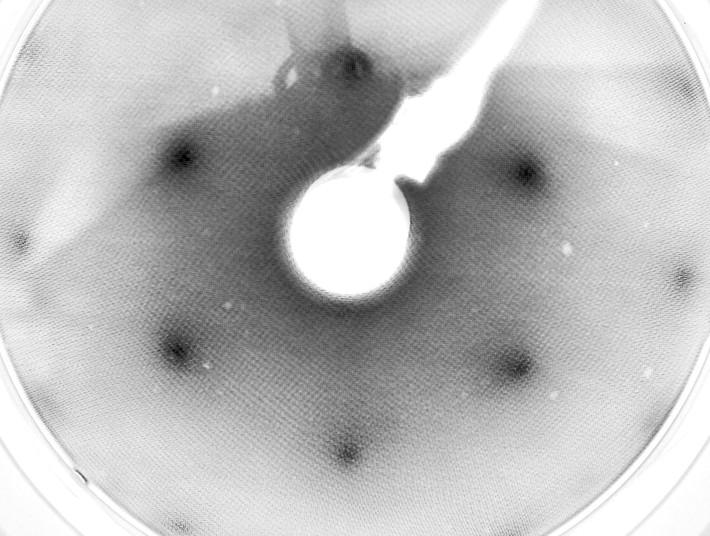
\includegraphics[width=\textwidth]{LEED-Bilder/bearbeitet/30ML_E208}
		\caption{\textit{30 Monolagen Au}}
		\label{Bild} 
	\end{minipage}
	\caption{noch eine Caption}
\end{figure}


\FloatBarrier
 
\section{Test des Dinges: Aufbringen von Molekül auf Substrat} \label{kaptest}
Der Aufbau zur Spraydeposition wurde an einer kleineren HV-Apparatur getestet (siehe \ref{testapparatur}). Der
Vorteil ist, dass diese Kammer wegen ihres kleineren Volumens schneller abgepumpt werden kann, was bei
auftretenden Problemen, bei denen man die Kammer öffnen muss, ein schnelleres Arbeiten ermöglicht.\\
Die sogenannte Testapparatur besteht aus zwei Pumpen (Vorpumpe (1) und Hauptpumpe (2)),
einer Hauptkammer mit Massenspektrometer (3) und Druckmessgerät bla (4) sowie dem aufgesetzten
Sprühbeschichter (4). Am Würfel des Beschichters ist eine (weitere) Membranpumpe angebracht (5). Das Ventil
zum Einspritzen des aufzutragenden Moleküls (6) wird angesteuert über ein Netzteil von IotaOne (7). Das
Substrat, hier zum Test ein Glasträger, befindet sich unterhalb des Beschichters (7.5) und kann durch einen
Fensterflansch beobachtet werden.\\
Die Ansteuerung des Ventils ermöglicht
prinzipiell zwei Modi: ein einmaliges Öffnen des
Ventils für einen einstellbaren Zeitraum (One
Shot Modus) und einen Zyklus von abwechselndem
Öffnen und Schließen des Ventils (Cycle Modus).
Da ein Einspritzen der Lösung in das Vakuum
natürlich den Druck steigen lässt, wurde hier
zunächst der Cycle Modus getestet, da so
mutmaßlich der Druck durch das Schließen des
Ventils zwischendrin besser erhalten werden
kann. In diesem Modus müssen die Dauern für das
Öffnen (On-Time) und des Schließens (Off-Time)
gewählt werden, wobei die Off-Time
betriebsbedingt mindestens so lang wie die
On-Time sein muss.\\
Beim Vakuumieren der Apparatur wurde Ventil 1
 geschlossen und Beschichter sowie die 
 Hauptkammer getrennt gepumpt, bis beide
 Vakuumpumpen jeweils vollständig hochgefahren
 waren.
 Um ein Druckgefälle zwischen Würfel und unterem
 Teil des Aufbaus herzustellen, getrennt durch den
 Konus, wurde dann Ventil 2 geschlossen und
 Ventil 1 geöffnet.
 Somit sollte innerhalb des Konus und dem
 Verbindungsstück darunter annähernd der gleiche
 Druck herrschen wie im Rest der Haupkammer.
 Nun konnte das gelöste Molekül über eine Pipette
 in das Reservoir des elektrischen Ventils
 eingefüllt und die On- sowie Off-Time gewählt
 werden.\\
Bei dem zum Testen zunächst benutzten Molekül
handelte es sich um Kupfer-2-phthalocyanin (kurz
CuPc), ein blauer Feststoff, der als Pigment
beispielsweise in Kunststoffen, Lacken oder
Druckerfarben verwendet wird. Das CuPc wurde in
dem farblosen organischen Lösungsmittel
Dimethylsulfoxid (kurz DMSO) aufgelöst, woraus
sich eine grobe Suspension ergab.\\ 
Der Versuch, On- und Off-Zeiten für das Ventil im
Bereich von wenigen Mikrosekunden einzustellen,
scheiterte, vermutlich wegen der Trägheit der Mechanik des
Ventils. Nachfolgend wurden sukzessive
On-Zeiten von 20, 30, 40ms mit jeweils gleich
langen Off-Zeiten getestet. Die Zyklendauern
wurden von 5s langsam auf bis zu 90s erhöht.
Hier offenbarten sich direkt Probleme mit der
Suspension: obwohl sich zu Beginn immerhin die
Spitze des Konus blau färbte, wurde
zwischenzeitlich scheinbar durch gröbere Partikel
in der Lösung die Öffnung des Ventils verstopft,
sodass auch bei längerer Zyklusdauer der Pegel im
Ventil konstant blieb. Um Ablagerungen auf dem
Ventil zu entfernen, wurde es mit DMSO ausgespült
und danach für den nächsten Zyklus mit reinem
DMSO befüllt. Nach dem zweiten Durchgang öffnete
sich das Ventil wieder, der Pegel sank.
Vermutlich konnte sich die Öffnung des Ventils
durch die Vibrationen während des Betriebs
"`freischütteln"'. Bei den nachfolgenden
Messungen war nach einer Zyklusdauer von etwa 20s
das Ventil leer, sodass nur noch Luft in die
Kammer gesogen wurde.
Längere Zyklen konnten also nur durchgeführt
werden, indem manuell während der Messung das
Ventil nachgefüllt wurde.
 
\begin{figure}[H]
	\centering
	\sffamily
	\includesvg[svgpath=testsb/]{sb}
	\caption{\textit{Der Aufbau des Sprühbeschichters.}}
\label{aufbau}
\end{figure}
 
Der Druck in der Hauptkammer war zu Beginn jedes
Zyklus im Bereich von $10^{-7}$ bis $10^{-6}$.
War die Öffnung des Ventils frei und konnte die
Lösung in die Kammer eintreten, fiel der Druck in
der Hauptkammer in den Bereich $10^{-4}$. Eine
Druckmessung im Würfel war zunächst nicht möglich.\\
Nach diversen Versuchen mit den genannten Parametern waren auf dem Glasträger kaum blaue Partikel zu
beobachten, im Würfel hatte sich jedoch auf dem Konus, dem Boden sowie den Seitenwänden eine blaue Schicht
gebildet. Zu diesem Zeitpunkt gab die Membranpumpe am Würfel eine Fehlermeldung, vermutlich war das
zu pumpende Gasvolumen, verursacht durch das DMSO, zu hoch. Gleichzeitig war zu vermuten, dass auch die
Öffnung des Konus verstopft sein könnte, also wurde der Würfel zunächst auseinandergebaut und gereinigt.\\
Beim Reinigen fiel auf, dass der Konus innen etwa auf dem ersten Centimeter eine blaue Schicht aufwies, der
Rest des Konus und der restliche Weg bis zum Glasträger wies keine augenscheinlichen Blaufärbungen auf. Die
nächste Idee war es, die CuPc-DMSO Lösung zu filtern, um grobe Partikel nicht mit in das Vakuum einzubringen.
Die vom Institut für Organische Chemie der Uni Mainz erhaltenen Filterpapiere waren jedoch  trotz gröbster
Stufe immer noch zu fein, sodass nach dem Filtern nur eine schwach bläuliche Flüssigkeit übrig blieb. Diese
Flüssigkeit wurde nicht getestet, da die Vermutung nahe lag, dass das Verhältnis Lösung zu Farbstoff zu hoch
war - und durch die viele Flüssigkeit nur die Pumpe belastet würde, ohne dass es das wenige CuPc bis zum
Glasträger schaffen würde.\\
Stattdessen wurde weiter die Suspension mit der gröberen Partikeln verwendet, jedoch die interne Vorpumpe im
Pumpstand für den Würfel abgeschraubt und eine andere, für höhere Gasvolumina ausgelegte Vorpumpe extern
angeschlossen. Zudem wurde die On-Time auf 1ms eingestellt, die Off-Time jedoch auf 50ms, später auf 100ms, um
den Druck insgesamt besser erhalten zu können. Außerdem wurde an den Würfel ein Druckmessgerät angeschlossen.
Bei den folgenden Messungen fiel der Druck von anfänglich $10^{-5}$ in den $10^{-3}$-Bereich in der
Hauptkammer, im Würfel schwankte der Druck hauptsächlich im $10^{-2}$-Bereich. Nach fünf Durchgängen war der
Strom bei beiden Pumpen auf über 2A gestiegen, sie somit also eine sehr hohe Leistung erbringen mussten, und
weiterhin war nichts auf dem Glasträger zu sehen.\\
Als nächstes wurde das Lösungsmittel getauscht, das DMSO wurde durch Dimethylformamid (kurz DMF) ersetzt,
da dieses das CuPc besser lösen sollte. Leider blieben noch immer grobe Partikel in der Lösung übrig. Weiterhin
wurden die On/Off-Zeiten geändert und die On-Time immer weiter verkürzt, bis zu 1ms On und 3s Off. Dies
bewirkte, dass innerhalb eines Ventil-auf-Ventil-zu-Zyklusses der Druck zwar anstieg bis in den
$10^{-3}$-Bereich, sich jedoch vor dem erneuten Öffnen des Ventils wieder in den Anfangsbereich $10^{-5}$
regulierte. Im Würfel schwankte der Druck wie vorher nur im mittleren $10^{-2}$-Bereich.\\
Nachdem sich immer noch keine sichtbare Schicht auf dem Glasträger absetzte, wurde der Aufbau kurzerhand
geändert: Ventil 1 wurde abgeschraubt und direkt
an den Zugang zum Pumpstand gelegt.
Kammer und Würfel können auf diese Weise zwar nicht mehr komplett getrennt gepumpt werden, jedoch sollte
weiterhin ein Druckgefälle von Würfel und Kammer möglich sein. Der Vorteil dieses Aufbaus ist, dass das bisher
notwendige Verbindungsstück zwischen großem Ventil und dem Adapterflansch wegfallen konnte, sich somit der Weg
zum Glasträger verkürzt. \\
 Da sich nach einem Versuch mit dem geänderten Aufbau die Öffnung des Konus zusetzte - der Druck in der
 Hautkammer änderte sich gar nicht mehr, sondern fiel immer weiter - wurde beschlossen, ein anderes Molekül als CuPc zu nehmen, da die
Parikel offensichtlich nur schlecht durch die Öffnung passen. Lösungsmittel, die es noch besser lösen könnten,
fallen unter die Kategorie stark gesundsheitsschädlich und sollten wegen mangelndem Abzug in diesem Fall nicht
verwendet werden.\\
Das nächste Lösungsmittel war Tetracyanochinodimethan (TCNQ), ein gelbfarbener, organische
Halbleiter, gelöst in Tetrahydrofuran (THF), wie die bisherigen Lösungsmittel ebenfalls ein
organisches Lösungsmittel. \\
Der erste Versuch lieferte bei einer On-Time von 1ms und einer Off-Time von 4s und einer
Gesamtdauer von 15min wiederum keine Farbablagerungen auf dem Glasträger. Der Druck ändert sich im
Würfel vom $10^{-2}$ in den $10^{-1}$mbar-Bereich, in der Kammer stieg er von $10^{-5}$ wieder auf $10^{-3}$mbar. Da der
Pumpstand, angezeigt durch hohen Strom und fallender Drehzahl, das Gasvolumen nicht verarbeiten
konnte, blieb es bei diesem Versuch mit diesen Parametern.\\
Mit der Vermutung, dass die Öffnung des Konus zu klein sein könnte, wurde dieser für die nächste
Messung komplett entfernt, ebenso die Anbindung an den mobilen Pumpstand. Nun war kein Druckgefälle
in Richtung des Glasträgers mehr vorhanden, dennoch sollte sich die Suspension ins Vakuum gebracht
verteilen und sich, so die Hoffnung, auch auf den Glasträger ablagern. Da nun das Gasvolumen durch
keine zusätzliche Pumpe mehr gepumpt werden konnte, wurde, um den Druck einigermaßen zu erhalten,
die On-Time auf 500µs erniedrigt, außerdem wurde zu zunächst der One-Shot-Modus eingestellt. Der
Druck stieg in der Kammer nur innerhalb des $10^{-5}$mbar-Bereiches an. Nach fünf Versuchen war auch
hier keine Beobachtung auf dem Glasträger zu machen. \\
Da auch der Würfel bei diesem Aufbau eigentlich nicht gebraucht wird, genauso wie die Ventile und
Verbindungen, konnte die Strecke zwischen Ventil und Glasträger weiter reduziert werden, indem der
Würfel komplett ausgebaut und das Ventil direkt auf den Adapterflansch über dem Glasträger befestigt
wurde. Außerdem wurden Edelstahlplättchen auf den
Glasträger geleget, da zur Vermutung stand, dass
das verwendete Molekül auf Glas nicht gut haftet.
Zuerst wurde getestet, bei welchen
Öffnungszeiten des Ventils der Druck innerhalb der Kammer vom Startwert (i. d. R $3\cdot10^{-5}$mbar) über den Druckanstieg zurück zum Startwert ging. Getestet wurden Zeiten in der Reihenfolge von 500, 300, 200, 250µs. Bei 200µs änderte sich der Druck in der Kammer gar nicht, sondern fiel weiter. Vermutlich lag auch diese On-Time außerhalb der mechanischen Reaktionsfähigkeit des Ventils. Die Zeiten bis zur
Erholung des Druckes lagen bei etwa 60s für 500µs, 50s für 300µs und stark schwankend zwischen 45s
und 70s für 250µs. Der Druck steig bei allen Versuchen auch nur innerhalb des
$10^{-5}$mbar-Bereiches an, je kürzer die On-Time, desto kleiner der Druckanstieg. Bei diesen
Versuchen war noch keine Beobachtung auf dem Glasträger zu machen. Um auszuschließen, dass dies an
der Kürze des Zeitintervalls lag, wurde eine lange Messung im Cycle-Modus über 1h und 15min
durchgeführt bei einer On-Time von 250µs und einer Off-Time von 70s, um den Druck über diesen
Zeitraum nicht konstant langsam zu steigern. Auch nach diesem Versuch war weder ein Gelbschimmer
auf dem Glasträger noch auf den Metallträgern zu sehen. Ob sich wenige Monolagen abgesetzt haben könnten, kann man durch diese
augenscheinliche Betrachtung nicht feststellen.\\




































% ____________________________________________________________________________
% \chapter{Zusammenfassung und Ausblick}
% Gold auf Re:





SB:
-Glasröhrchen in ventil, um mehr flüssigkeit reintun zu können (wenn über langen zeitraum viel riengemacht
werden muss), spritzschutz
-ausrichtung substrat in molekülkammer - sichtfenster weg! markierung an magnet?
-konus oben spitzer machen? damit keine tropfenbildung auf "`terasse"'? oder konus oben vergrößern?
-filtern der lösung oder verdünnen? geht filtern auch mit größeren molekülen?
-zum säubern muss ventil abgeschraubt werden, da nicht erreichbares reservoir direkt über öffnung
-evtl weg verkürzen mit kürzerem zwischenstück
-weitere test mit quarzwaage zur skalierung? bzw groben abschätzung, da jedes molekül anderes
gewicht



%_______________________________________________________________________________
% \begin{appendix}
% \chapter{Anhang}
% 
% \section{Tabellen und Abbildungen}
% 
% 
% 
% %_______________________________________________________________________________
% \section{Weiterf\"uhrende Details zur Arbeit}



%_______________________________________________________________________________


\bibliography{literatur}{}
\bibliographystyle{alpha}



%_______________________________________________________________________________
% \chapter{Danksagung}
% 
% ... an wen auch immer. Denken Sie an Ihre Freundinnen und Freunde, 
% Familie, Lehrer, Berater und Kollegen.
% 
% \end{appendix}

\end{document}  
        
        